\documentclass{svproc}
\usepackage{graphicx,amsmath,amssymb,booktabs,url,float}
\usepackage[T1]{fontenc}
\usepackage[utf8]{inputenc}
\usepackage{newtxtext,newtxmath}
\usepackage[hidelinks]{hyperref}
\graphicspath{{../figures/}}
\begin{document}
\mainmatter
\title{Generative Structural Programs for Evidence-Weighted Causal Path Explanations}
\titlerunning{Generative Structural Programs and Causal Paths}
\author{Anonymous submission draft}
\authorrunning{Anonymous}
\institute{Author information withheld}
\maketitle
\begin{abstract}
Narrative causal explanations require more than a directed graph: interventions depend on executable mechanisms, and overlapping paths cannot be added as independent causes. We present an auditable prototype in which a local language model proposes variables, dependencies and typed structural expressions from a frozen document packet. A restricted evaluator checks mechanisms, freezes them during interventions and attributes an explicit reference-to-model contrast to a fixed collection of paths. Shared edges activate once through set union, while evidence support remains separate from structural influence. We evaluate the system on 60 independently generated structural causal models, with grouped development, calibration and test splits and deterministic text variants. Held-out scores for direct, graph-conditioned, single-model and compatible-rule methods were 0.677, 0.590, 0.693, 0.786, respectively. Gains depend on mechanism completeness; the overall paired interval versus direct prompting includes zero. The three television-continuity application networks contain ten, eight and three nodes. Every retained path includes an unsupported mechanism, making the evidence-weighted segment ranking uninformative. Formal execution and exact attribution therefore do not establish source-valid literary explanations. Failures, generated assumptions and raw completions are retained. No human review, comprehension improvement or calibrated probability of war is claimed. The artifact supports inspection of model-dependent explanations and exposes the additional evidence and researcher review needed for scientific conclusions.
\keywords{structural causal models, narrative reasoning, program synthesis, evidence provenance, path attribution}
\end{abstract}

\section{Introduction}
A narrative can describe events without identifying the mechanisms that connect them. A graph records possible dependencies, but generally cannot determine what follows from an intervention. Even with executable mechanisms, overlapping explanatory paths share junctions and may interact or inhibit one another. Adding independent path scores therefore need not reconstruct the modeled outcome.

We study an integration of source-bounded language-model extraction, restricted structural-program synthesis, executable interventions, and a specified path-coalition game. The objective is an inspectable collection of evidence-weighted paths converging on a declared conflict outcome. We do not claim that structural causal models, equation synthesis, narrative graphs, or Shapley attribution are individually new. The contribution assessed here is their operational integration, controlled evaluation, and explicit separation of evidential support from modeled influence.

This is an evidence-backed research draft. Literary mechanisms are hypotheses and require researcher adjudication. Computational consistency does not establish causal identification, and the controlled benchmark is not independent validation of a fictional historical interpretation.

\section{Related work}
Bynum and Cho define sequence-driven structural causal models with language-model mechanisms and user-supplied structure~\cite{bynum}. Our prototype instead asks the model to propose both structure and bounded executable mechanisms from a source packet. LLM-SR uses language-model priors and program search for scientific equation discovery~\cite{shojaee}; our textual observations usually cannot identify coefficients or choose a unique structural law. Linguistic graph generation~\cite{li} and semantic-relation event reasoning~\cite{koupaee} establish closely related narrative tasks. Yamin et al. document tensions between world knowledge and source-specific causal reasoning~\cite{yamin}, motivating the explicit refusal to treat model memory as retrieved evidence. Shadow-Loom uses typed narrative world models with language models at extraction and rendering boundaries~\cite{wilmot}; this close integration precedent limits broad novelty claims.

Shapley Flow incorporates graph structure into attribution~\cite{wang}. Do-Shapley quantifies intervention-based contributions~\cite{jung}, PWSHAP studies targeted path-wise explanation~\cite{terminassian}, and Witter et al. provide exact do-Shapley computation techniques~\cite{witter}. Our game uses fixed reference inputs on inactive focused edges and paths as players. It is not asserted to equal these estimands or a natural path-specific effect. Its allocation depends on the chosen paths, reference values, structural programs and background scenario.

\section{Method}
\subsection{Source-linked structural programs}
Given a frozen document packet $\mathcal D$ and outcome definition $Q$, the language model proposes $M=(\mathcal V,\mathcal U,\mathcal F,\mathcal R)$, with $X_i=f_i(X_{\mathrm{Pa}(i)},U_i)$. The registry $\mathcal R$ stores operational definitions, state types, actor and temporal context, source identifiers, exact short-span offsets, assumptions, reference values, and failures. No distribution over $\mathcal U$ is invented. Application results condition on explicitly recorded factual background states.

Expressions are JSON abstract syntax trees with declared parent/background leaves and bounded arithmetic, comparisons, logical operators, conditionals and a sigmoid. The evaluator has no import, filesystem, network or unrestricted code-execution facility. It limits tree size/depth and execution time, checks domains, acyclicity, temporal consistency, graph/expression agreement, active dependence and factual compatibility. Dependence checks are exhaustive on small finite domains and explicitly sampled otherwise. Interventions replace only the targeted equation and reuse the same background across factual and modified worlds.

Each artifact can receive at most two diagnostic repairs within a recorded protocol. Failed completions and exploratory protocol revisions are retained. No application-specific reason, edge, or structural equation is researcher-authored. Direct source offsets establish occurrence of a quoted span, not independent semantic entailment.

\subsection{Evidence support}
For each application edge, the model assesses event support, mechanism explicitness, temporal compatibility, contradiction and corroboration. A scalar $c_e\in[0,1]$ is a heuristic evidence score, not a probability of causation. Controlled display weights instead use binary rule availability from the extracted missing-rule flag. Secondary summaries from the same editorial family do not provide independent corroboration. The score is never multiplied into structural equations. An unfilled human-review form is supplied; no human assessment is reported.

\subsection{Shared-edge path aggregation}
A predeclared source-balanced, shortest-first rule retains at most eight root-to-outcome paths; all paths and omitted edges are recorded. For coalition $S$, let $E(S)=\bigcup_{p\in S}E(p)$ and $E_F=\bigcup_pE(p)$. Focused inactive edges supply explicit reference parent values to child functions; edges outside $E_F$ stay active. In the fixed factual background $u$, define
\begin{equation}
v_M(S)=W_{M_{E(S)}}(u),\qquad
\phi_p=\mathbb E_{\sigma}[v_M(\mathrm{Pre}_\sigma(p)\cup\{p\})-v_M(\mathrm{Pre}_\sigma(p))].
\end{equation}
Shared edges execute once through set union. We cache effective edge masks. Controlled games use exact enumeration up to six paths and otherwise 64 permutations with paired backgrounds. Final application games use exact enumeration up to eight paths, retaining their initial sampled allocations for audit. Permutation standard errors concern numerical sampling, not structural uncertainty. The allocation obeys
\begin{equation}
v_M(\mathcal P)=v_M(\varnothing)+\sum_{p\in\mathcal P}\phi_p.
\end{equation}
Edge unions can enable recombined routes, which are reported. The game describes a mechanism-ablation contrast, not independently isolated paths or actionable interventions. We compare declared references, model-derived references from jointly intervening on boundary events, and domain-endpoint stress tests. Coalition execution keeps the factual background even for the model-derived reference policy. We also group overlapping paths into disjoint mechanism components. A naive standalone-path sum is retained only as a diagnostic.

A path's display support is $c_p=\min_{e\in p}c_e$, with geometric-mean sensitivity. Supporting source clusters split a unit evidential allocation $a_{\ell p}$. Segment priority is $R_\ell=\sum_pa_{\ell p}c_p|\phi_p|$. Unsupported paths receive no fabricated segment. This is evidence retrieval priority, not the effect of deleting narrative text.

\section{Experimental design}
\subsection{Controlled benchmark and comparisons}
The generator creates 60 independent deterministic Boolean SCMs: 20 each with 12, 18 and 24 variables, half with an omitted local mechanism. Chains, shared ancestors, convergences, conjunction, redundancy, exclusive alternatives and inhibition occur in the generating family. A traceable deterministic renderer states the available rules and factual settings. Missing-rule uncertainty enumerates all active two-parent Boolean functions compatible with those observations. This family is exhaustive under its local deterministic assumptions, not under arbitrary confounding.

Splits contain 12 development, 12 calibration and 36 test SCMs. Each test SCM has a matched connective paraphrase and paragraph-order variant. Eight questions cover factual states, interventions, shared-background counterfactuals, joint interventions, ancestry and mechanism availability. Both text variants remain in the same split. Verification is automated; texts are comparatively explicit controlled descriptions, not representative open-domain prose. The benchmark evaluates reconstruction of named states and mechanisms; it does not independently validate open-ended literary concept discovery. Application development used several disclosed revisions after monolithic and modular generations failed. The final source-first protocol extracts atomic claims from short source chunks, rejects malformed claims, audits actor/action entailment, and lets the model select dependencies one child at a time from source-ordered eligible earlier events. Research-question endpoints are explicit and separate from the later documentary horizon. Context outside the outcome ancestry is excluded rather than linked to satisfy a size target. Root states have explicit background identities; each endogenous expression is synthesized against named parent slots. Every artifact permits at most two repairs within its protocol, but total development attempts across protocols exceed that bound and are retained. The application protocol is therefore not an untouched test of the controlled generation configuration.

B0 answers from the text. B1 receives the identical text and extracted adjacency list. B2 executes the first admissible candidate. P reuses that candidate and enumerates compatible local rules for a flagged missing mechanism. Application P also retains generated mechanism alternatives and evidence/path annotations. B0/B1 use equal 2,048-token answer caps; synthesis can use 4,096 tokens. Actual input tokens differ because B1 includes the graph, and extraction/repair costs are shared, not charged twice. A1 makes evidence display weights uniform without altering equations. A2 sums standalone path effects. No calibration map is fitted or transferred to the literary application.

For identified queries, the score requires the correct outcome set. For underidentified binary queries, explicit abstention or $\{0,1\}$ is accepted. Interventions, uncertainty handling and extraction are also exported separately. Paired differences and 2,000-resample percentile intervals use independent SCMs after averaging their variants. Inference failures count as unsuccessful queries; admitted-only graph metrics are descriptive and subject to selection.

\subsection{Television application and source gate}
The frozen corpus contains 32 television episode plot summaries and 241 passage segments. Only Plot sections are used; book-adaptation production notes are excluded. Access attempts to HBO's synopsis and the television wiki failed. These are explicitly secondary, dependent summaries. Their URLs, access dates, content hashes, normalized-text offsets and frozen retrieval memberships are retained; the copyrighted full-text packet is excluded from release.

The outcomes concern early armed conflict between the northern/Riverlands coalition and the Lannister-controlled crown; the northern campaign against Bolton rule; and continuation of Daenerys's conquest through the assault on King's Landing. Actor scope, episode horizon and onset/continuation meaning are frozen in configuration. Robert's Rebellion was replaced before generation because accessible retrospective passages did not sufficiently establish its onset mechanisms. The northern case covers coalition formation and sustained conflict, not merely one battle. Counterfactual answers have no observable literary gold labels.

\subsection{Compute and reproducibility}
The primary model is Qwen3-14B-AWQ, revision \texttt{31c69efc29464} (full hash in the run manifest), served on one RTX 4090 with vLLM 0.10.2, an 8,192-token context, two-request concurrency, 0.88 memory utilization, temperature 0.2 and top-$p$ 0.8. Thinking is disabled for the frozen controlled protocol and enabled for the revised application source/mechanism review; all returned reasoning tokens count toward compute. A 20-request pilot produced 20 valid JSON responses; 3 of eight initial synthesis candidates were executable. Median and 90th-percentile request times were 17.29 and 30.73 seconds. Raw failures include incompatible initial tokenizer dependencies, an inherited download setting, malformed AST leaves and application-generation errors. Only the isolated project environment was changed.

An absolute 24-hour deadline, a project process-group watchdog, per-request checkpoints and 20-minute local synchronization bounded execution. The target is completion within 22 hours. Requests and generated artifacts are cached by revision, prompt/source hashes, settings and seed. Complete usage, environment versions and actual final runtime are in the accompanying run manifest. Cost is not estimated without billing evidence.

\section{Measured results}
Held-out scores for direct, graph-conditioned, single-model and compatible-rule methods were 0.677, 0.590, 0.693, 0.786, respectively.
The paired B2--B0 difference is 0.016 (95\% cluster bootstrap interval [-0.099, 0.125]).
\begin{table}[t]
\centering\caption{Held-out query scores; intervals resample independent SCMs.}
\begin{tabular}{lrrl}\toprule Method & SCMs & Score & 95\% interval \\\midrule
B0 & 36 & 0.677 & [0.623, 0.731] \\
B1 & 36 & 0.590 & [0.536, 0.646] \\
B2 & 36 & 0.693 & [0.580, 0.806] \\
P & 36 & 0.786 & [0.675, 0.885] \\
\bottomrule\end{tabular}\end{table}

\begin{figure}[t]\centering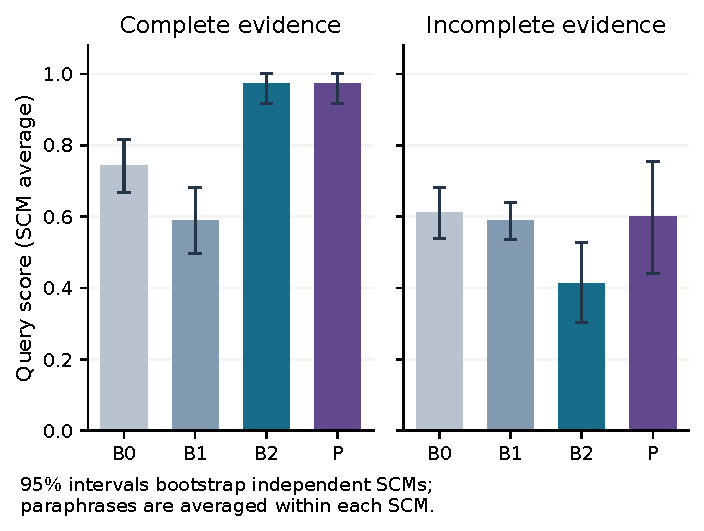
\includegraphics[width=\linewidth]{benchmark_performance.pdf}\caption{Paired test conditions; text variants are averaged within SCM.}\label{fig:benchmark}\end{figure}
Figure~\ref{fig:benchmark} separates complete and incomplete evidence conditions.
Across 120 completed text/seed records, 92 initial candidates were valid and 100 had an admissible model after bounded repair. These counts concern generated records, not additional independent datasets. The full CSV distinguishes extraction, identified intervention accuracy and uncertainty handling. Positive controlled scores cannot establish the correctness of literary mechanisms.

Evidence completeness changes the conclusion. B2 minus B0 is 0.229 [0.118, 0.330] with complete mechanisms, but -0.198 [-0.333, -0.066] with an omitted mechanism. P recovers some uncertainty handling by retaining compatible rules. Its overall difference from B0 is 0.109 [-0.021, 0.229]; the interval includes zero, so these data do not establish an overall improvement over direct prompting.

On the held-out texts, 53 of 72 models were initially admissible and 59 were admissible after repair. Among admitted models only, mean edge precision and recall were 1.000 and 1.000, and specified nonroot local function agreement was 0.9988. These reconstruction diagnostics condition on successful synthesis and exclude missing mechanisms; they do not compensate for failed records in the primary score.

A2 failed the aggregation identity on 26 of 59 admitted test texts: 20 naive sums exceeded the full/reference contrast and 6 fell below it. The maximum absolute discrepancy was 3.000, versus a maximum path-coalition efficiency residual of 0. This checks an algebraic property of the specified game, not historical validity.

For A1, the paired difference in source-support nDCG@5 between evidence weighting and uniform weighting was -0.0006 [-0.1112, 0.0866] across 22 eligible SCMs. No clear ranking improvement is established. Relevance labels identify available support on generated influential paths; they are not independent ground truth for causal importance.

A post-hoc dataset diagnostic also limits interpretation: 63 of 90 complete-condition intervention/counterfactual queries retain the factual outcome. In the incomplete condition, all 43 identified structural queries retain it, while 47 are ambiguous. Simply carrying forward the observed outcome therefore scores 0.70 on identified complete structural queries and 1.00 on identified incomplete ones. This was not a predeclared inference baseline, and its denominator differs from the main eight-query score. Future evaluation should include more identified, outcome-changing interventions under incomplete evidence.

The predeclared seed subset contains the first two test SCM identifiers from each size/completeness stratum, using original texts only. It has 36 of 36 planned records over seeds 2027, 2028 and 2029, with all seeds available for 12 of 12 SCMs. The main table remains restricted to the primary seed; repeated seeds are not independent narratives.

Within the fully repeated subset, the mean within-SCM P score range across seeds is 0.083. The seed-averaged paired P--B0 difference is 0.205 [-0.049, 0.427], bootstrapping SCMs. This smaller-subset sensitivity analysis does not replace the primary comparison.



\begin{table}[t]\centering\caption{Accepted generations / distinct functional signatures and principal-network size. Repeated functions do not add independent models or evidence.}
\begin{tabular}{lrrrr}\toprule Conflict & Gen./unique & Nodes & Edges & Paths \\\midrule
five kings & 2/1 & 10 & 13 & 6 \\
northern campaign & 1/1 & 8 & 12 & 6 \\
daenerys conquest & 1/1 & 3 & 2 & 2 \\
\bottomrule\end{tabular}\end{table}

\begin{table}[t]\centering\caption{Principal-model source/mechanism audit. Span matches are mechanical checks; partial-event and edge-status judgments come from the same LLM. E/I/U denote explicit, inferred and unsupported or unassessed mechanisms. These are not human labels.}\label{tab:audit}
\begin{tabular}{lrrl}\toprule Conflict & Valid spans & Partial events & Edges E/I/U \\\midrule
five kings & 11/11 & 1 & 0 / 1 / 12 \\
northern campaign & 9/9 & 1 & 0 / 5 / 7 \\
daenerys conquest & 4/4 & 1 & 0 / 0 / 2 \\
\bottomrule\end{tabular}\end{table}
Table~\ref{tab:audit} separates traceable event spans from mechanism support. A source can describe an event without identifying its outgoing equation.

Only one distinct functional signature was obtained per case. The repeated Five Kings generation is functionally equivalent and does not provide alternative-mechanism robustness. The northern and Daenerys networks miss the ten-node target, despite a broader generated inventory. These shortfalls reflect source compression and construction failures as well as limited primary-source access. No graph was padded. The source-coverage pass and corrected complete-packet outcome retrieval are retained as exploratory revisions, independent of final numerical performance.

Every retained principal path contains an unsupported mechanism. Its weakest-link support is therefore zero, and every evidence-weighted segment priority is zero. The artifact exposes influential but weakly supported paths, but does not establish a useful source ranking for these applications. Uniform weighting supplies a separate display ablation; it cannot create evidential support.

The northern model's node c01 introduces the alias ``Edmure Tully (the Blackfish)'', although the personal name is absent from the entire frozen packet. The same-model source reviewer nevertheless accepted the claim. A post-hoc literal alias-coverage flag retains this discrepancy without supplying a corrected identity or changing the equation. This selected example is not a measured population error rate, but demonstrates that model critique is not independent entailment verification. Conversely, a critique can misread an episode code; its flags are unresolved review items, not automatically true corrections.
Measured campaign duration is 5.99 hours through the recorded analysis endpoint, with 5.67 hours of model-service residency and peak sampled memory of 21996.0 MiB. The server recorded 935619.0 generated tokens, including interrupted requests where counted. Concurrent request durations are not added as GPU wall time; no billing cost is inferred.
\subsection{War of the Five Kings}
Figure~\ref{fig:five_kings} shows the principal model and its source/equation identifiers.
The principal model contains 10 variables and 13 edges; 6 retained paths cover 100.0\% of its edges. Its reference outcome is 0.000 and full outcome is 1.000; path shares sum to 1.000. The naive standalone sum is 0.000. The attribution efficiency residual is 1.11e-16. These are modeled contrasts in fixed factual backgrounds, not war probabilities.
Final automated source critique: \{"partial": 1, "supported": 9\}. Timing flagged as contradicted: W. Reference-semantics flags: e12\_5, W. Duplicate-event flags: 0. Per-node parent-order fields remain unresolved for 2 nodes. 0 of 2 explanations passed the same-model full-text trace audit. These checks are not independent adjudication; flagged claims remain unresolved in this frozen hypothesis.
The retained model provides 12 canonical single or paired reference-intervention queries. Matched text/graph baselines use the same frozen packet; agreement with modeled outcomes is descriptive, not literary accuracy.
p1 follows Ned orders Gregor's arrest and summons Tywin $\rightarrow$ Tywin's forces attack Riverrun $\rightarrow$ Campaign outcome. Its allocated contribution is 0.167 and weakest-link support is 0.000.
p2 follows Joffrey's parentage revelation $\rightarrow$ Robert's altered will $\rightarrow$ Stark men slaughtered by City Watch $\rightarrow$ Robb calls Northern banners to war $\rightarrow$ Campaign outcome. Its allocated contribution is 0.167 and weakest-link support is 0.000.
\begin{figure}[p]\centering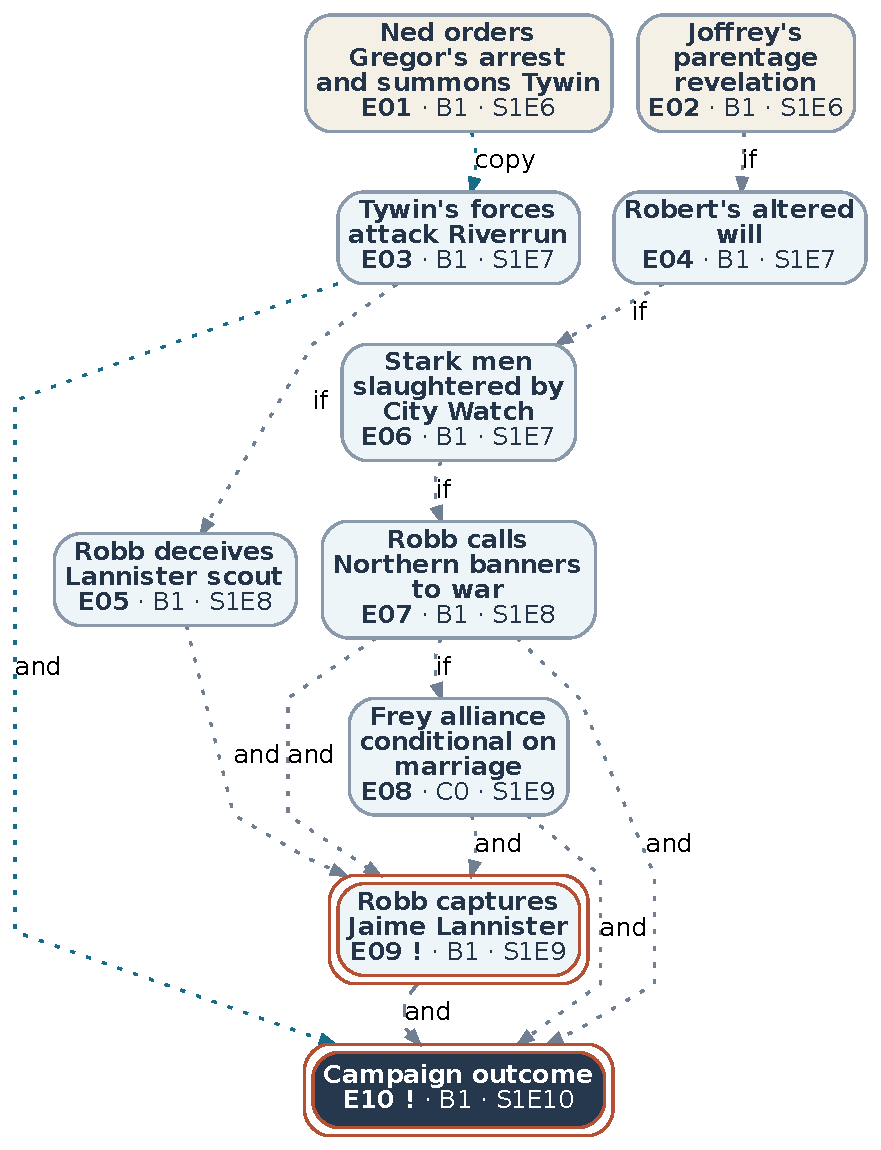
\includegraphics[width=\linewidth,height=.85\textheight,keepaspectratio]{five_kings_network.pdf}\caption{War of the Five Kings: generated hypothesis. Cream nodes are background boundaries; the dark node is the outcome. B/C mark Boolean/categorical states; E links nodes to equations. Episode labels record time. Dashed edges are inferred, dotted edges unsupported. Teal highlights one maximum-share path (ID breaks ties); double borders mark shared junctions. ! marks an unresolved source flag. Edge style encodes support, not influence; widths are uniform.}\label{fig:five_kings}\end{figure}
\subsection{Northern campaign against Bolton rule}
Figure~\ref{fig:northern_campaign} shows the principal model and its source/equation identifiers.
The principal model contains 8 variables and 12 edges; 6 retained paths cover 100.0\% of its edges. Its reference outcome is 0.000 and full outcome is 1.000; path shares sum to 1.000. The naive standalone sum is 0.000. The attribution efficiency residual is 1.11e-16. These are modeled contrasts in fixed factual backgrounds, not war probabilities.
This schema does not meet the planned ten-node principal-network target. It is retained as an executable smaller hypothesis rather than enlarged with unsupported links.
Final automated source critique: \{"supported": 8\}. Timing flagged as contradicted: none. Reference-semantics flags: none. Duplicate-event flags: 0. Per-node parent-order fields remain unresolved for 5 nodes. 0 of 1 explanations passed the same-model full-text trace audit. These checks are not independent adjudication; flagged claims remain unresolved in this frozen hypothesis.
The retained model provides 12 canonical single or paired reference-intervention queries. Matched text/graph baselines use the same frozen packet; agreement with modeled outcomes is descriptive, not literary accuracy.
p1 follows Ramsay's threat to Castle Black $\rightarrow$ Sansa's unilateral declaration $\rightarrow$ Campaign outcome. Its allocated contribution is 0.167 and weakest-link support is 0.000.
p2 follows Ramsay's threat to Castle Black $\rightarrow$ Sansa's unilateral declaration $\rightarrow$ Littlefinger's manipulation of Robin Arryn $\rightarrow$ Campaign outcome. Its allocated contribution is 0.167 and weakest-link support is 0.000.
\begin{figure}[p]\centering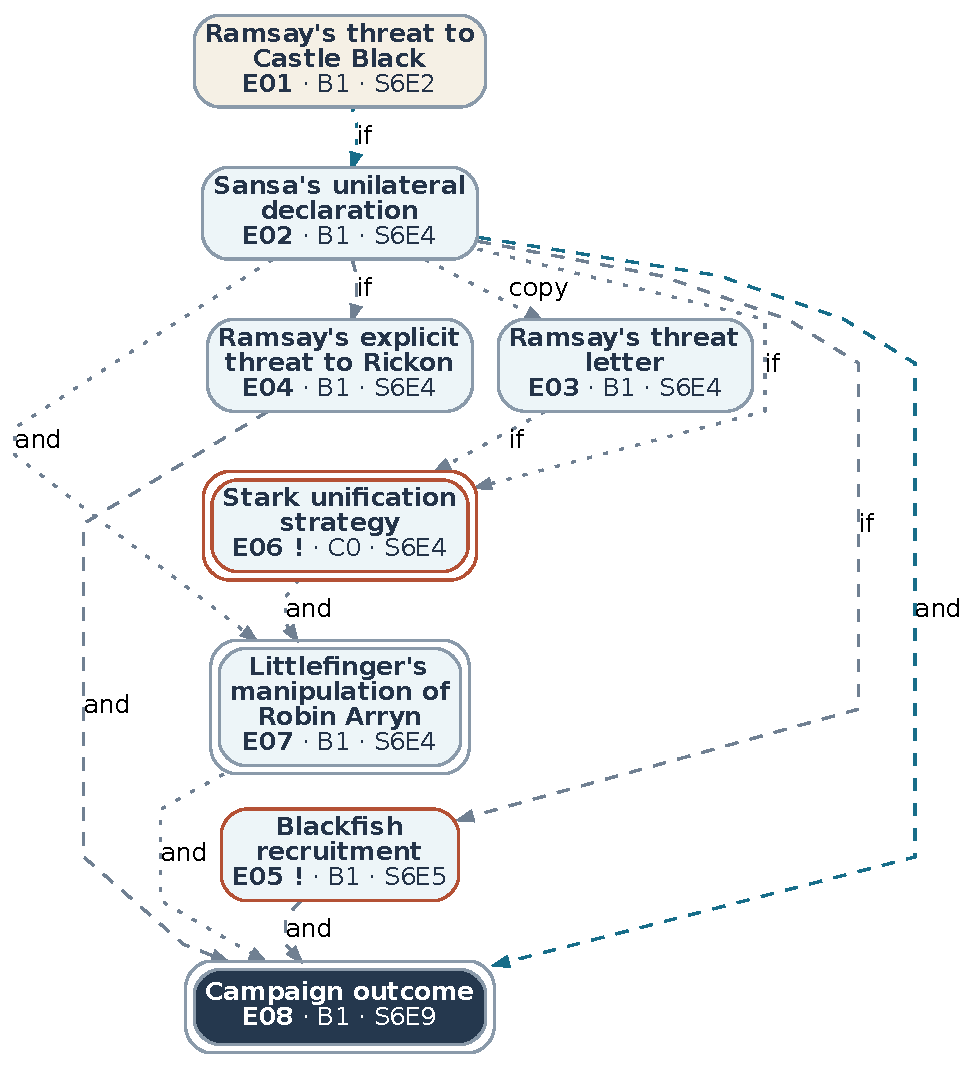
\includegraphics[width=\linewidth,height=.85\textheight,keepaspectratio]{northern_campaign_network.pdf}\caption{Northern campaign against Bolton rule: generated hypothesis. Cream nodes are background boundaries; the dark node is the outcome. B/C mark Boolean/categorical states; E links nodes to equations. Episode labels record time. Dashed edges are inferred, dotted edges unsupported. Teal highlights one maximum-share path (ID breaks ties); double borders mark shared junctions. ! marks an unresolved source flag. Edge style encodes support, not influence; widths are uniform.}\label{fig:northern_campaign}\end{figure}
\subsection{Daenerys's conquest of Westeros}
Figure~\ref{fig:daenerys_conquest} shows the principal model and its source/equation identifiers.
The principal model contains 3 variables and 2 edges; 2 retained paths cover 100.0\% of its edges. Its reference outcome is 0.000 and full outcome is 1.000; path shares sum to 1.000. The naive standalone sum is 0.000. The attribution efficiency residual is 0. These are modeled contrasts in fixed factual backgrounds, not war probabilities.
This schema does not meet the planned ten-node principal-network target. It is retained as an executable smaller hypothesis rather than enlarged with unsupported links.
Final automated source critique: \{"partial": 1, "supported": 2\}. Timing flagged as contradicted: W. Reference-semantics flags: W. Duplicate-event flags: 0. Per-node parent-order fields remain unresolved for 0 nodes. 0 of 1 explanations passed the same-model full-text trace audit. These checks are not independent adjudication; flagged claims remain unresolved in this frozen hypothesis.
The retained model provides 3 canonical single or paired reference-intervention queries. Matched text/graph baselines use the same frozen packet; agreement with modeled outcomes is descriptive, not literary accuracy.
p1 follows Iron Fleet destruction of Daenerys' ships $\rightarrow$ Campaign outcome. Its allocated contribution is 0.500 and weakest-link support is 0.000.
p2 follows Cersei's forces execute Missandei $\rightarrow$ Campaign outcome. Its allocated contribution is 0.500 and weakest-link support is 0.000.
\begin{figure}[ht]\centering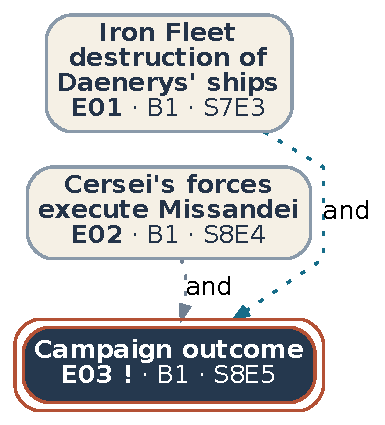
\includegraphics[width=.60\linewidth,height=.85\textheight,keepaspectratio]{daenerys_conquest_network.pdf}\caption{Daenerys's conquest of Westeros: generated hypothesis. Cream nodes are background boundaries; the dark node is the outcome. B/C mark Boolean/categorical states; E links nodes to equations. Episode labels record time. Dashed edges are inferred, dotted edges unsupported. Teal highlights one maximum-share path (ID breaks ties); double borders mark shared junctions. ! marks an unresolved source flag. Edge style encodes support, not influence; widths are uniform.}\label{fig:daenerys_conquest}\end{figure}
Figure~\ref{fig:paths} decomposes the modeled contrast, Figure~\ref{fig:paired} shows a fixed-mechanism intervention, and Figure~\ref{fig:sensitivity} shows reference dependence. Exact allocation removes permutation error, but leaves structural and source uncertainty unresolved. In these models, jointly derived boundary references preserve the declared allocation, while the alternative domain-endpoint contrast produces zero allocations. All retained routes are covered, with no additional recombined routes; grouping overlapping paths gives one mechanism component for Five Kings and the northern campaign, and two for Daenerys. These observations concern the retained models, not universal invariance properties.
\begin{figure}[t]\centering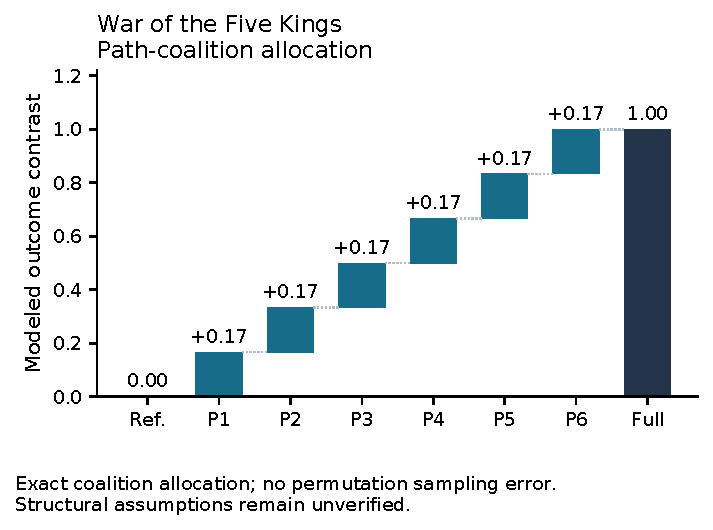
\includegraphics[width=\linewidth]{path_contributions.pdf}\caption{Path shares reconstruct the explicit reference-to-model contrast.}\label{fig:paths}\end{figure}
\begin{figure}[p]\centering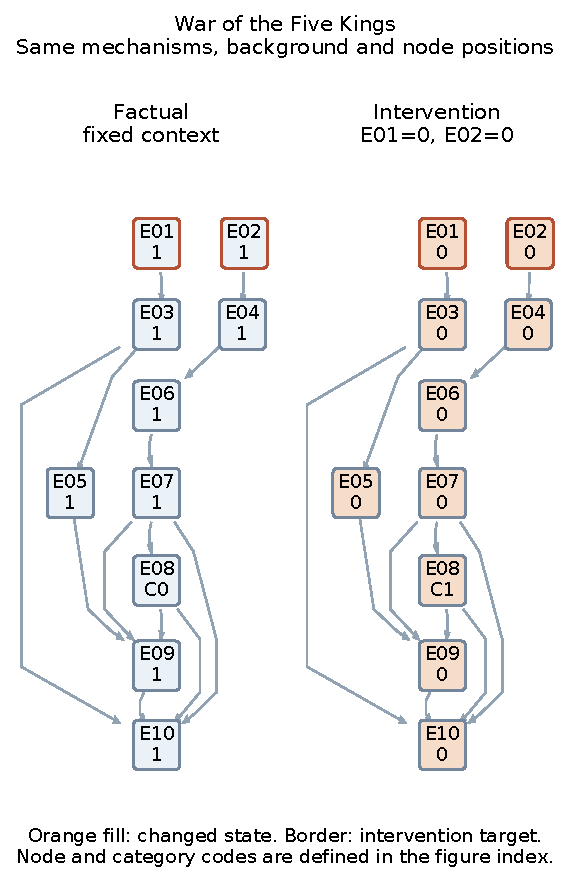
\includegraphics[width=\linewidth,height=.84\textheight,keepaspectratio]{paired_counterfactual.pdf}\caption{Paired Five Kings worlds use identical node positions, edge routes and fixed mechanisms. E codes match the principal network; the index supplies full definitions.}\label{fig:paired}\end{figure}
\begin{figure}[t]\centering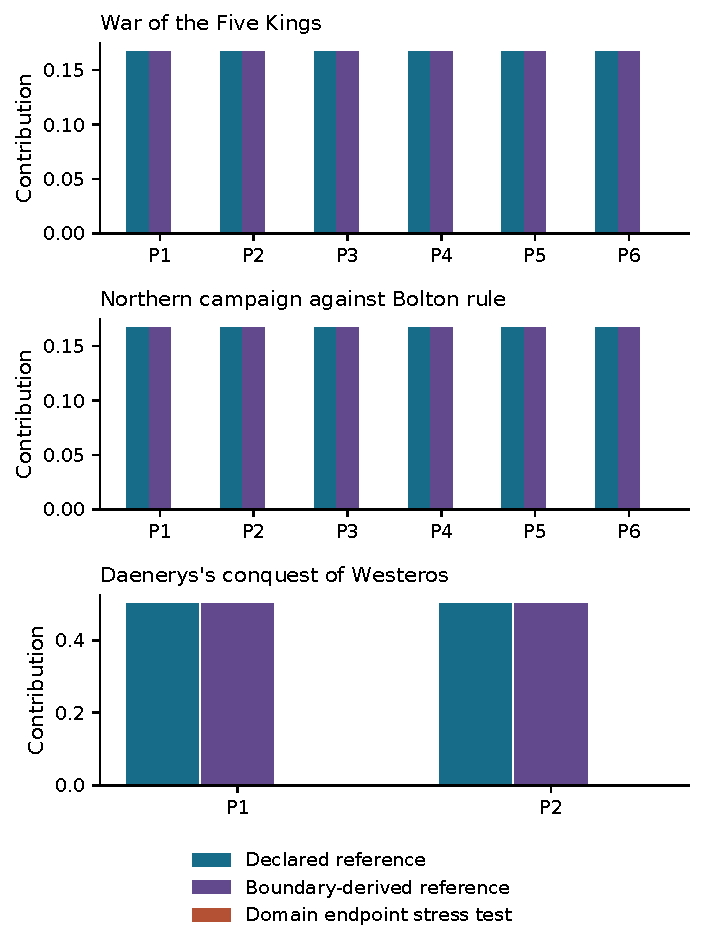
\includegraphics[width=\linewidth]{reference_sensitivity.pdf}\caption{Reference changes alter the path game; endpoint stress tests need not be historically plausible.}\label{fig:sensitivity}\end{figure}

\section{Limitations and required scientific review}
The benchmark has a deliberately bounded logical family and highly explicit prose. Graph generation and functional equivalence outside that family are not established. The calibration split is kept separate but no probabilistic evidence calibration is claimed. A single primary model and limited decoding seeds do not characterize all model variability. B1 benefits from shared extraction and is a graph-conditioned language-model baseline rather than a pure graph algorithm.

Application observations rarely identify conjunction, redundancy, coefficients, hidden common causes or alternative histories. Root backgrounds are explicit context assumptions, not estimated independent disturbances. Source summaries can omit, compress or misstate an episode; multiple summaries in this corpus do not constitute independent corroboration. Model-generated event and mechanism assessments require independent review. Our exact-span audit measures traceability, not factual correctness. A short matching citation can be insufficient to entail a longer claim.

A fixed path collection omits graph context and can activate recombined routes. Shared-edge handling prevents duplicate execution but does not make an allocation uniquely true. Reference sensitivity and disjoint-mechanism grouping are required interpretation checks. Alternate domain endpoints are stress tests, not automatically meaningful historical counterfactuals. Negative shares indicate inhibitory model effects, not moral blame. Path shares must not be summed again along an edge chain.

No reader study was conducted. Figure readability and interpretability are design objectives, not measured comprehension improvements. No independent human review, causal probabilities, significance claims, or literary counterfactual gold outcomes are invented. An anonymous review form and per-edge source audit accompany the artifact. A researcher must check source entailment, outcome scope, plausible mechanisms, source licensing and the interpretation of all tables before submission.

Generated explanations are retained separately from the numerical trace. The final audit rejects every retained explanation, including structured-field failures, spurious quotation of audit instructions and unsupported claims of a uniquely strongest path. Failed prose is withheld from display. The manuscript's numerical descriptions are derived from verified execution records and do not certify the generated free text. A second model, independent application seed repetitions, evidence-guided selection ablation and interactive explorer were deferred under the output-token budget; none is represented as completed.

\section{Conclusion}
The prototype makes generated assumptions executable and inspectable, separates support from influence, and tests an overlapping-path allocation against controlled models. Its strongest warranted conclusions concern formal execution, observed benchmark behavior and sensitivity of specified model contrasts. Establishing source-valid literary causal explanations remains a separate scientific task.

\section*{Declaration on Generative AI}
An AI coding assistant implemented and ran the prototype, analyzed artifacts and drafted this manuscript from a researcher-supplied plan. Qwen3-14B-AWQ generated experimental variables, graphs, mechanisms, evidence assessments and explanations. This document is an unsubmitted scaffold for human scientific review; no human validation or final author approval is asserted. Human authors must develop, critically review and take responsibility for scientific arguments and conclusions in accordance with the conference policy. AI systems are not authors.

\clearpage
\begin{thebibliography}{12}
\bibitem{bynum} Lucius E.J. Bynum; Kyunghyun Cho: Language Models as Causal Effect Generators. Proceedings of the 2025 Conference on Empirical Methods in Natural Language Processing, 2025. \url{https://aclanthology.org/2025.emnlp-main.107/}.
\bibitem{shojaee} Shojaee, Parshin; Meidani, Kazem; Gupta, Shashank; Barati Farimani, Amir; Reddy, Chandan: LLM-SR: Scientific Equation Discovery via Programming with Large Language Models. International Conference on Learning Representations, 2025. \url{https://proceedings.iclr.cc/paper_files/paper/2025/hash/28df8e730c054c5331855fd4d5403ba9-Abstract-Conference.html}.
\bibitem{li} Zehan Li; Ruhua Pan; Xinyu Pi: Beyond LLMs A Linguistic Approach to Causal Graph Generation from Narrative Texts. Proceedings of the 7th Workshop on Narrative Understanding, 2025. \url{https://aclanthology.org/2025.wnu-1.10/}.
\bibitem{koupaee} Mahnaz Koupaee; Xueying Bai; Mudan Chen; Greg Durrett; Nathanael Chambers; Niranjan Balasubramanian: Causal Graph based Event Reasoning using Semantic Relation Experts. Proceedings of the 63rd Annual Meeting of the Association for Computational Linguistics (Volume 1: Long Papers), 2025. \url{https://aclanthology.org/2025.acl-long.1269/}.
\bibitem{yamin} Yamin, Khurram; Gupta, Shantanu; Ghosal, Gaurav; Lipton, Zachary; Wilder, Bryan: LLMs Struggle to Balance Reasoning and World Knowledge in Causal Narrative Understanding. International Conference on Learning Representations, 2026. \url{https://proceedings.iclr.cc/paper_files/paper/2026/hash/98741856b327ec2f9503179398da662f-Abstract-Conference.html}.
\bibitem{wilmot} Wilmot, David: Shadow-Loom: Causal Reasoning over Graphical World Models of Narratives. arXiv preprint 2605.02475, 2026. \url{https://arxiv.org/abs/2605.02475}.
\bibitem{wang} Jiaxuan Wang; Jenna Wiens; Scott Lundberg:  Shapley Flow: A Graph-based Approach to Interpreting Model Predictions . International Conference on Artificial Intelligence and Statistics, 2021. \url{https://proceedings.mlr.press/v130/wang21b.html}.
\bibitem{jung} Yonghan Jung; Shiva Kasiviswanathan; Jin Tian; Dominik Janzing; Patrick Bloebaum; Elias Bareinboim: On Measuring Causal Contributions via do-interventions. International Conference on Machine Learning, 2022. \url{https://proceedings.mlr.press/v162/jung22a.html}.
\bibitem{terminassian} Lucile Ter-Minassian; Oscar Clivio; Karla Diazordaz; Robin J. Evans; Christopher C. Holmes: PWSHAP: A Path-Wise Explanation Model for Targeted Variables. International Conference on Machine Learning, 2023. \url{https://proceedings.mlr.press/v202/ter-minassian23a.html}.
\bibitem{witter} R. Teal Witter; Álvaro Parafita; Tomas Garriga; Maximilian Muschalik; Fabian Fumagalli; Axel Brando; Lucas Rosenblatt: Exactly Computing do-Shapley Values. International Conference on Machine Learning, 2026. \url{https://proceedings.mlr.press/v306/witter26a.html}.
\end{thebibliography}
\end{document}
